\section{Figury}

\noindent Zapomniałeś wzoru lub definicji? Nic sie nie martw! 

\maketitle StudUnity posiada zakładkę "Przypominajka", w której zawarte są najpotrzebniejsze wzory matematycze, fizyczne i nie tylko. Uważasz że jakiegoś brakuje? Śmiało wyślij do nas wiadomość lub prześlij swój pomysł rozwiązania tego problemu. Żadna wiadomość nie zostanie pominięta!


\begin{figure}[htbp]
    \centering
    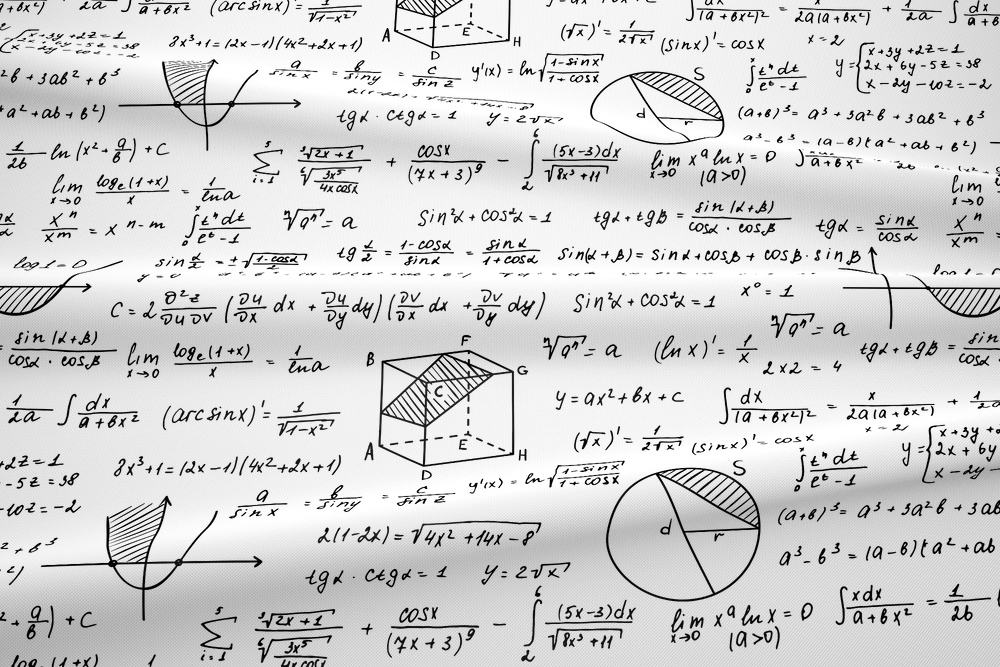
\includegraphics[width=0.7\textwidth]{pictures/wzory.jpg}
    \caption{Wzory}
    \label{fig:Wzory}
\end{figure}